\capitulo{5}{Aspectos relevantes del desarrollo del proyecto}

\section{Entorno de desarrollo}
Como entorno de desarrollo de los prototipos hemos utilizado Jupyter, ya que en sus notebooks interactivos puedes ejecutar directamente código Python como si fuese un intérprete.
Y Eclipse mas PyDev, como IDE, para programar en clases y paquetes de forma mas cómoda.
\subsection{Ventajas}
\begin{itemize}
\item He podido añadir widgets para calibrar en buen grado las funciones que hemos utilizado.
Gracias a estos widgets podemos dar valores e ir viendo como cambia la salida de la función de forma interactiva. Como podemos observar en la imagen \ref{fig:5.1}.

\begin{figure}[h]
\centering
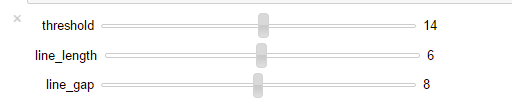
\includegraphics[width=0.65\textwidth]{Widget}
\caption{Ejemplo de un widget sobre la función de Hough}
\label{fig:5.1}
\end{figure}

\item Su rápida visualización sin tener grandes conocimientos de interfaz gráfica ha sido un gran apoyo para poder visualizar desde el principio las imágenes procesadas y como quedaban. Como podemos observar en la imagen \ref{fig:5.2}. 

\begin{figure}
\begin{subfigure}[b]{.5\linewidth}
\centering\large 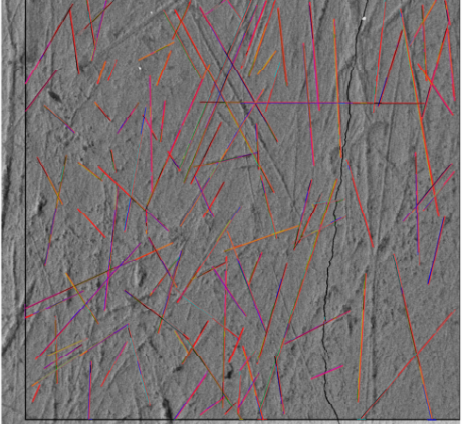
\includegraphics[width=.9\textwidth]{ComparativaLineas2}
\caption{Líneas antes de unir}
\end{subfigure}%
\begin{subfigure}[b]{.5\linewidth}
\centering\large 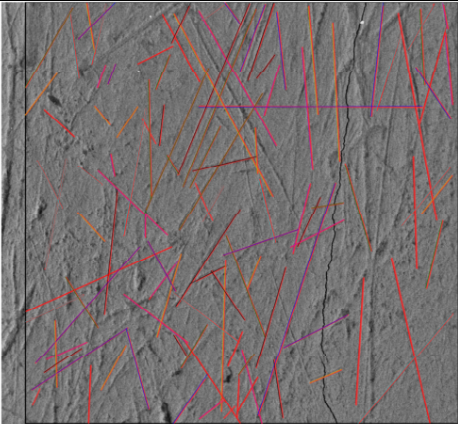
\includegraphics[width=.9\textwidth]{ComparativaLineas1}
\caption{Líneas después de unir}
\end{subfigure}
\caption{Ejemplo de una visualización del resultado intermedio de las funciones.}\label{fig:5.2}
\end{figure}


\item Desde el propio entorno puedes ejecutar, no solo código estructurado en script, sino también código estructurado en clases y llamadas a métodos es como un IDE pero con limitaciones. Como podemos observar en la imagen \ref{fig:5.3}.

\begin{figure}[h]
\centering
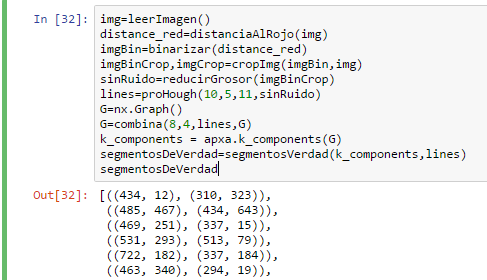
\includegraphics[width=0.65\textwidth]{Ejecucion}
\caption{Ejemplo de una ejecución.}
\label{fig:5.3}
\end{figure}

\item Multitud de librerías y funciones que en entornos parecidos como Matlab serian de pago y aquí al ser software libre el ejemplo anterior lo resume en una librería Numpy \cite{Numpy}.
\end{itemize}

\section{Procesado imagen}
Para llegar a conseguir calcular las líneas que había pintadas en las imágenes, tube que realizar una serie de pasos que vamos a resumir en tres etapas.
\subsection{Binarización}
Partiendo de una imagen que solo tenía líneas, en cualquier color, pintadas encima de las estrías producidas por el desgaste y lo demás de la imagen en escala de grises. Lo primero fue leer la imagen a través de las funciones ya programadas en la librería de Scikit-Image (skimage) \cite{scik:skeleton}.
Una vez que tenemos la imagen guardada en el espacio de color RGB podemos empezar el procesado, transformando la imagen al espacio de color CIELAB, partiendo de este espacio calcularemos la distancia de los pixeles al color seleccionado por el usuario.

Calculamos la distancia de cada pixel de la imagen al color deseado, pasamos la imagen de distancias a blanco y negro y así tendremos un valor entre 0 y 256 en cada pixel correspondiente a la distancia al color. Cuanto mas alejado mas negro y los que sean del color, en blanco.

Para que la diferencia sea blanco o negro binarizamos, la imagen con un valor umbral así los valores de la distancia que sean mayores que el umbral pasaran a valer máximo y los que no consigan pasar el umbral serán los bordes blancos, como podemos observar en la figura \ref{fig:5.4}.


\begin{figure}
\begin{subfigure}[c]{.5\linewidth}
\centering\large 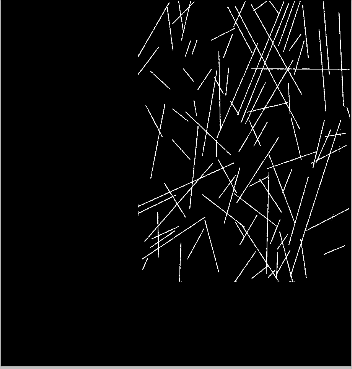
\includegraphics[width=.9\textwidth]{paso1Binariza}
\caption{Original}
\end{subfigure}%
\begin{subfigure}[c]{.5\linewidth}
\centering\large 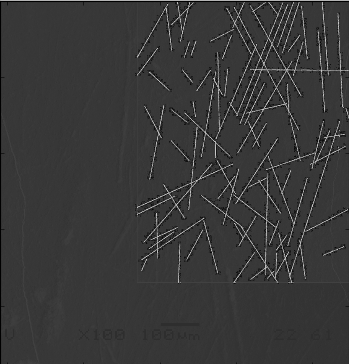
\includegraphics[width=.9\textwidth]{paso1DistanciaR}
\caption{Distancia al rojo}
\end{subfigure}
\begin{subfigure}[c]{.5\linewidth}
\centering\large 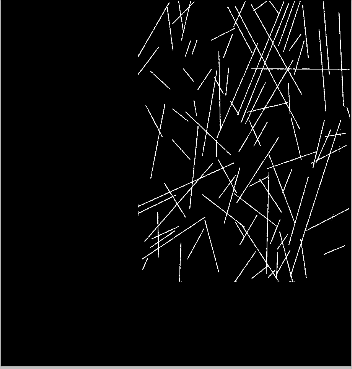
\includegraphics[width=.9\textwidth]{paso1Binariza}
\caption{Imagen binarizada}
\end{subfigure}
\caption{Resumen visual binarización.}\label{fig:5.4}
\end{figure}


\subsection{Obtener segmentos}
Partimos de la imagen binarizada y lo primero es reducir el grosor de las líneas detectadas a un pixel, eso lo conseguimos llamando a la función skeletonize que nos devuelve la imagen con las líneas de un pixel (así no acumulamos errores y es mas rápida la búsqueda de rectas).\\
Seguidamente llamamos a la función <<probabilistic hough line>> que nos va a encontrar segmentos que formaran las líneas el funcionamiento ha sido explicado en el apartado (conceptos teóricos). Como podemos observar en la figura \ref{fig:5.5}.


\begin{figure}
\begin{subfigure}[c]{.5\linewidth}
\centering\large 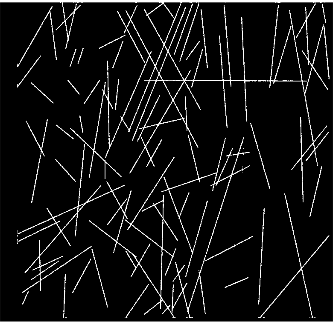
\includegraphics[width=.9\textwidth]{paso2Binaria}
\caption{Binarizada}
\end{subfigure}%
\begin{subfigure}[c]{.5\linewidth}
\centering\large 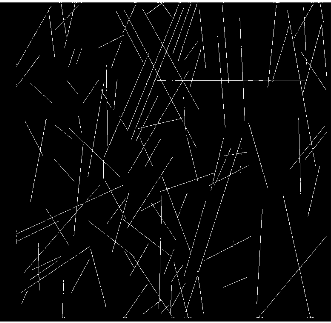
\includegraphics[width=.9\textwidth]{Paso2Skele}
\caption{líneas a 1 pixel}
\end{subfigure}
\begin{subfigure}[c]{.5\linewidth}
\centering\large 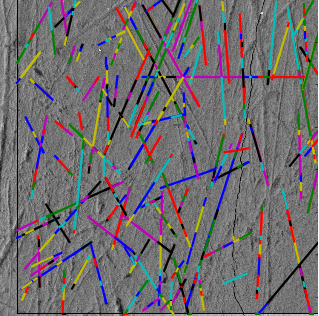
\includegraphics[width=.9\textwidth]{Paso2Segmentos}
\caption{Imagen original con segmentos}
\end{subfigure}
\caption{Resumen visual Obtener Segmentos.}\label{fig:5.5}
\end{figure}

\subsection{Procesado de segmentos}
Llegados a este punto, lo que tenemos son:
\begin{itemize}
\item Muchos segmentos que forman las líneas reales y tenemos que unirlos. Para ello vamos a usar la teoría de grafos añadiendo los segmentos a un grafo.

\item Para unir dos segmentos tiene que cumplirse que la distancia mínima entre sus extremos sea menor que un umbral y si pasa este punto comprobaremos que el angulo que forman entre ellas sea menor a otro umbral.

\item Si cumplen las dos condiciones añadiremos un camino al grafo desde la recta uno a la recta dos como se ve en la figura \ref{fig:5.6}.
\end{itemize}


\begin{figure}
\begin{subfigure}[b]{.5\linewidth}
\centering\large 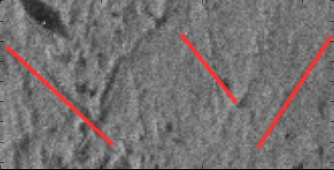
\includegraphics[width=.9\textwidth]{grafoLineasOri}
\caption{Imagen con segmentos en rojo.}
\end{subfigure}
\begin{subfigure}[b]{.5\linewidth}
\centering\large 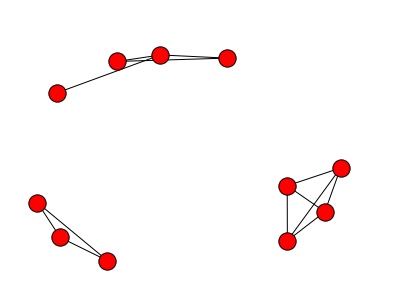
\includegraphics[width=.9\textwidth]{grafo}
\caption{Grafo de clusters de segmentos.}
\end{subfigure}
\caption{Resumen visual procesado de Segmentos.}\label{fig:5.6}
\end{figure}

\subsection{Recuperación de líneas}
Ahora lo que tenemos es un grafo con clusters, ya que cada cluster se identifica con únicamente una recta y tendremos tantos como rectas.
Un problema de grafos es el problema de las k-componentes pero a nosotros solo nos interesan las 1-componentes del grafo ya que cada grupo de estos segmentos cercanos se corresponde con una recta real.
Devolvemos la combinación de los segmentos mas relevantes de cada cluster y estos se convierten en nuestra buscada linea real, como podemos observar en la figura \ref{fig:5.7}.
\begin{figure}[h]
\centering
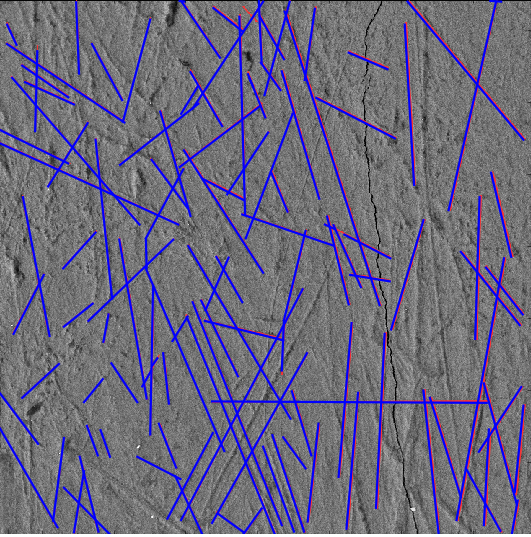
\includegraphics[width=0.65\textwidth]{ResultanteDelGrafo}
\caption{Líneas obtenidas después de procesar el grafo}
\label{fig:5.7}
\end{figure}

\subsection{Resumen pasos}

\begin{itemize}
\item Binarizar la imagen para solo quedarnos con los objetos de interés
\item Obtener segmentos que forman trozos de las líneas.
\item Añadir caminos entre las líneas cercanas en un grafo.
\item Obtener los grupos de líneas próximas y devolver la recta que las una. 
\end{itemize}

\section{Interfaz}
La programación de interfaces en Python ha sido bastante sencillo y muy intuitiva, por lo que lo recomendamos para futuras ocasiones.

En grandes rasgos estoy bastante contento con PyQt5 me ha resultado muy útil y la librería de Matplotlib también ya que con ellas he conseguido resolver todos los problemas planteados.

\section{Internacionalización}

En nuestra aplicación, hemos implementado una funcionalidad para traducirla a los dos idiomas, que hemos considerado mas apropiados para el usuario, ya que los usuarios serán españoles pero publicaran los artículos en Ingles.

La forma de implementarlo ha sido mediante una clase, donde se guardan los string correspondientes a los textos en inglés y otra en español. Mediante un fichero de configuración, se guarda el idioma usado, en el fichero y así una vez cambiado quedara como configuración. Para futuras ejecuciones sin necesidad de cambiar cada vez el idioma, si lo queremos volver a cambiar este fichero quedara también cambiado.

\section{Artículo}
Partiendo de este proyecto, se va a realizar una articulo para una revista científica que aun no sabemos a cual en particular va a ser enviado dicho articulo porque las fechas en las que se ha terminado el articulo no han sido las mas acordes.

Pero no obstante si que se va a realizar y enviar a una revista científica un articulo de este proyecto.
